% blog-title: Martingales and Optional Stopping
% blog-date: 2026-06-18
% blog-description: A polished note on martingales, stopping times, Ville's inequality, e-processes, and why bandit proofs need filtrations.
% blog-lang: en

\documentclass[en,nofont,11pt]{elegantbook}

\title{Martingales and Optional Stopping}
\subtitle{Why Bandit Proofs Need Filtrations}
\author{Tang}
\institute{Tang's Machine Learning Blog}
\date{2026-06-18}
\version{1.0.0}
\bioinfo{Topic}{Martingales, Optional Stopping, Bandit Theory}
\cover{assets/blog-cover.jpg}

\usepackage{fontspec}
\ifdefined\setCJKmainfont
\else
  \usepackage[UTF8,scheme=plain,fontset=none]{ctex}
\fi
\usepackage{xcolor}
\usepackage{listings}
\usepackage{float}
\usepackage{tcolorbox}
\tcbuselibrary{breakable, listings, skins}
\usetikzlibrary{arrows.meta,positioning,calc,decorations.pathmorphing,decorations.pathreplacing,fit,backgrounds,patterns,shapes.geometric}

\IfFontExistsTF{Microsoft YaHei}{
  \setCJKmainfont{Microsoft YaHei}
  \setCJKsansfont{Microsoft YaHei}
  \setCJKmonofont{Microsoft YaHei UI}
}{
  \IfFontExistsTF{Noto Serif CJK SC}{
    \setCJKmainfont{Noto Serif CJK SC}
    \setCJKsansfont{Noto Sans CJK SC}
    \setCJKmonofont{Noto Sans Mono CJK SC}
  }{}
}

\definecolor{blogAccent}{HTML}{1F6F8B}
\definecolor{blogInk}{HTML}{172026}
\definecolor{blogCodeBg}{HTML}{F5F7F8}
\definecolor{blogCodeBorder}{HTML}{D6E2E8}
\definecolor{blogKeyword}{HTML}{B23A48}
\definecolor{blogString}{HTML}{287D4F}
\definecolor{blogComment}{HTML}{687783}

\lstdefinestyle{blogcode}{
  basicstyle=\ttfamily\small,
  keywordstyle=\bfseries\color{blogKeyword},
  stringstyle=\color{blogString},
  commentstyle=\itshape\color{blogComment},
  numberstyle=\scriptsize\color{blogComment},
  numbers=left,
  numbersep=8pt,
  showstringspaces=false,
  breaklines=true,
  tabsize=2,
  columns=fullflexible,
  keepspaces=true
}

\newtcblisting{codeblock}[2][]{
  listing only,
  breakable,
  enhanced,
  colback=blogCodeBg,
  colframe=blogCodeBorder,
  arc=2mm,
  boxrule=0.4pt,
  left=6mm,
  right=2mm,
  top=1mm,
  bottom=1mm,
  listing options={style=blogcode, language=#2},
  #1
}

\hypersetup{
  colorlinks=true,
  linkcolor=blogAccent,
  urlcolor=blogAccent,
  citecolor=blogAccent
}

\addbibresource{tex/bandits-references.bib}

\definecolor{martingaleBlue}{RGB}{28,73,135}
\definecolor{martingaleLightBlue}{RGB}{232,241,252}
\definecolor{martingaleOrange}{RGB}{150,75,25}
\definecolor{martingaleLightOrange}{RGB}{255,247,236}
\definecolor{martingaleGreen}{RGB}{38,105,65}
\definecolor{martingaleLightGreen}{RGB}{235,247,239}
\definecolor{martingaleGray}{RGB}{247,247,247}
\colorlet{mainblue}{martingaleBlue}
\colorlet{lightblue}{martingaleLightBlue}
\colorlet{deeporange}{martingaleOrange}
\colorlet{lightorange}{martingaleLightOrange}
\colorlet{deepgreen}{martingaleGreen}
\colorlet{softgreen}{martingaleLightGreen}
\colorlet{lightgray}{martingaleGray}

\newtcolorbox{keyidea}[1][]{enhanced,breakable,colback=lightblue,colframe=mainblue,
  coltitle=white,fonttitle=\bfseries,title=Key idea,#1}
\newtcolorbox{thinkbox}[1][]{enhanced,breakable,colback=lightorange,colframe=deeporange,
  coltitle=white,fonttitle=\bfseries,title=Think,#1}
\newtcolorbox{resultbox}[1][]{enhanced,breakable,colback=white,colframe=mainblue,
  coltitle=white,fonttitle=\bfseries,title=Result,#1}
\newtcolorbox{patternbox}[1][]{enhanced,breakable,colback=softgreen,colframe=deepgreen,
  coltitle=white,fonttitle=\bfseries,title=Proof pattern,#1}

\newcommand{\E}{\mathbb{E}}
\newcommand{\Pbb}{\mathbb{P}}
\newcommand{\R}{\mathbb{R}}
\newcommand{\one}{\mathbf{1}}
\newcommand{\F}{\mathcal{F}}
\newcommand{\G}{\mathcal{G}}
\newcommand{\Var}{\operatorname{Var}}
\newcommand{\argmax}{\operatorname*{arg\,max}}
\newcommand{\st}{\text{subject to}}

\begin{document}
\maketitle
\frontmatter
\tableofcontents
\mainmatter

\chapter{A Decision Rule Also Chooses When to Look}

Suppose an online experiment compares two recommendation policies. Every few minutes the dashboard refreshes. The new policy is slightly ahead. The lead disappears, returns, and grows again. Someone says:

\begin{center}
\emph{``Let us stop as soon as the result looks convincing.''}
\end{center}

Nothing about that sentence is unusual. In fact, it is exactly what a sequential learner should do: look at the data, decide whether enough has been learned, and either continue or stop.

The difficulty is more subtle. A confidence interval designed for a fixed sample size answers a fixed-time question:
\[
\text{``What can happen at time }n\text{?''}
\]
A sequential procedure asks a different question:
\[
\text{``What can happen at any time at which the data persuade us to stop?''}
\]
Those are not the same event.

A bandit algorithm is full of such random times. It may stop exploring an arm when its upper confidence bound becomes small. It may eliminate an action when the evidence is strong enough. It may end an experiment once one action is clearly best. The amount of data collected is therefore not fixed in advance. It is produced by the data themselves.

\begin{keyidea}
The word \emph{adaptive} means more than ``the next action depends on the past.'' It also means that the amount of data, the arm being sampled, and the time at which a conclusion is reached may all depend on the past.
\end{keyidea}

Martingales are the language that keeps this dependence honest \cite{williams1991probability,lattimore2020bandit}. They do not make adaptivity disappear. They separate it into two pieces:
\[
\boxed{\text{a choice made from the past}}
\qquad+
\qquad
\boxed{\text{new noise whose conditional mean is zero}.}
\]
Once this separation is visible, many proofs become simple bookkeeping.

\section{The first warning: peeking changes the event}

Let $X_1,X_2,\ldots$ be Bernoulli observations with mean $1/2$. At a fixed time $n$, an exact one-sided test can be calibrated so that
\[
\Pbb_{1/2}(\text{reject at time }n)\le 0.05.
\]
Now imagine applying a fresh $5\%$ test after every observation and stopping at the first rejection. The event is no longer
\[
\{\text{reject at time }n\}.
\]
It is
\[
\bigcup_{t=1}^{n}\{\text{reject at time }t\}.
\]
Even when each individual event is rare, their union need not be rare.

This is not a technicality. It is the central reason fixed-time probability statements cannot simply be reused after arbitrary monitoring.

\begin{thinkbox}
Optional stopping is often summarized as ``stopping does not create profit in a fair game.'' That slogan is useful, but incomplete. The theorem only works when the stopping rule and the process satisfy conditions that prevent rare, enormous outcomes from carrying hidden expectation.
\end{thinkbox}

\chapter{The Past as a Mathematical Object}

Before defining a martingale, we need a clean way to say what is known at each moment.

At the beginning of round $t$, the learner has seen everything from the previous rounds. Call this information $\F_{t-1}$. Using only this information, the learner chooses an action $A_t$. Then the reward $X_t$ arrives, and the information grows to $\F_t$.

\begin{center}
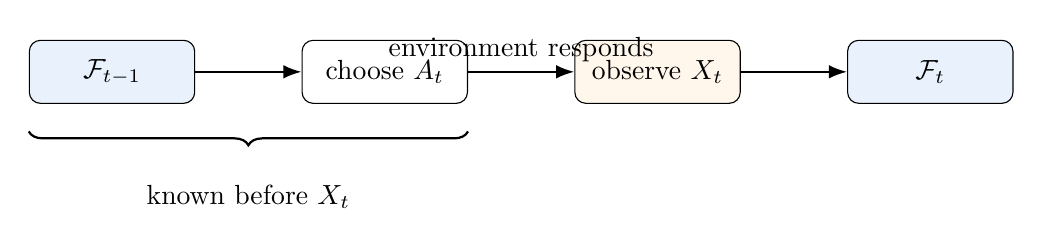
\begin{tikzpicture}[>=Latex,node distance=1.35cm]
\node[draw,rounded corners,fill=lightblue,minimum width=2.1cm,minimum height=0.8cm] (past) {$\F_{t-1}$};
\node[draw,rounded corners,fill=white,minimum width=2.1cm,minimum height=0.8cm,right=of past] (act) {choose $A_t$};
\node[draw,rounded corners,fill=lightorange,minimum width=2.1cm,minimum height=0.8cm,right=of act] (rew) {observe $X_t$};
\node[draw,rounded corners,fill=lightblue,minimum width=2.1cm,minimum height=0.8cm,right=of rew] (new) {$\F_t$};
\draw[->,thick] (past) -- (act);
\draw[->,thick] (act) -- node[above]{environment responds} (rew);
\draw[->,thick] (rew) -- (new);
\draw[decorate,decoration={brace,amplitude=5pt,mirror},thick] ($(past.south west)+(0,-0.35)$) -- ($(act.south east)+(0,-0.35)$)
 node[midway,below=0.55cm]{known before $X_t$};
\end{tikzpicture}
\end{center}

The sequence
\[
\F_0\subseteq \F_1\subseteq \F_2\subseteq\cdots
\]
is called a \emph{filtration}. The inclusion simply says that information accumulates. Yesterday's facts do not become unknown today.

\section{Adapted and predictable}

A process $Y_t$ is \emph{adapted} when $Y_t$ is known by time $t$. In symbols, $Y_t$ is $\F_t$-measurable.

A process $H_t$ is \emph{predictable} when $H_t$ is known just before round $t$. In discrete time, this means $H_t$ is $\F_{t-1}$-measurable.

The distinction is small in notation and decisive in proofs:
\[
\underbrace{A_t}_{\text{chosen before reward}}
\quad\text{is predictable,}
\qquad
\underbrace{X_t}_{\text{revealed after action}}
\quad\text{is adapted but not predictable.}
\]

A legal bandit policy cannot choose $A_t$ using $X_t$, because $X_t$ has not yet happened. That simple chronological fact is exactly what predictability records.

\section{Conditional expectation means ``average after using the past''}

The ordinary mean $\E[X_t]$ averages over every possible history. The conditional mean
\[
\E[X_t\mid \F_{t-1}]
\]
first freezes the past and then averages only over what remains random.

For a stochastic bandit with arm means $\mu_1,\ldots,\mu_K$, once $A_t$ has been chosen we have
\[
\E[X_t\mid \F_{t-1}]
=
\mu_{A_t}.
\]
This equation does not say the reward equals $\mu_{A_t}$. It says that after all past information and the current action are known, the remaining uncertainty has mean $\mu_{A_t}$.

\chapter{Martingales: Fairness After Conditioning on the Past}

A martingale is often introduced through gambling. The useful idea is simpler:

\begin{center}
\emph{After using everything already known, the next expected change is zero.}
\end{center}

Let $M_0,M_1,M_2,\ldots$ be an adapted process with finite expectations. It is a martingale when
\[
\E[M_t\mid \F_{t-1}]=M_{t-1}
\qquad\text{for every }t\ge 1.
\]
Subtract $M_{t-1}$ from both sides:
\[
\E[M_t-M_{t-1}\mid \F_{t-1}]=0.
\]
If we write
\[
D_t=M_t-M_{t-1},
\]
then
\[
\boxed{\E[D_t\mid \F_{t-1}]=0.}
\]
The sequence $D_t$ is called a \emph{martingale difference sequence}.

\begin{keyidea}
The condition is not that the increments are independent. The condition is weaker and better suited to sequential learning: after conditioning on the entire past, the next increment has mean zero.
\end{keyidea}

\section{The simple random walk}

Let $\xi_t\in\{-1,+1\}$ be a fair coin step:
\[
\Pbb(\xi_t=1)=\Pbb(\xi_t=-1)=\frac12.
\]
Define
\[
S_t=\sum_{s=1}^{t}\xi_s,
\qquad S_0=0.
\]
Then
\begin{align*}
\E[S_t\mid\F_{t-1}]
&=\E[S_{t-1}+\xi_t\mid\F_{t-1}]\\
&=S_{t-1}+\E[\xi_t\mid\F_{t-1}]\\
&=S_{t-1}+0\\
&=S_{t-1}.
\end{align*}
So $S_t$ is a martingale.

Notice what the equation does \emph{not} say. It does not say the path stays near zero. A fair random walk may wander far upward or downward. Martingale fairness concerns conditional expectation, not pathwise calmness.

\section{The noise in a bandit is a martingale difference}

Let $A_t$ be the arm selected at round $t$, and let $X_t$ be its reward. Define the centered reward
\[
D_t=X_t-\mu_{A_t}.
\]
Then
\begin{align*}
\E[D_t\mid\F_{t-1}]
&=\E[X_t-\mu_{A_t}\mid\F_{t-1}]\\
&=\E[X_t\mid\F_{t-1}]-\mu_{A_t}\\
&=\mu_{A_t}-\mu_{A_t}\\
&=0.
\end{align*}
Therefore
\[
M_t=\sum_{s=1}^{t}(X_s-\mu_{A_s})
\]
is a martingale.

This is the first important research pattern:

\begin{patternbox}
Write an adaptive observation as
\[
\text{observation}
=
\text{conditional mean given the past}
+
\text{martingale noise}.
\]
The policy may be highly adaptive. The centered noise can still have conditional mean zero.
\end{patternbox}

\chapter{Predictable Multipliers: How Adaptivity Enters Safely}

Suppose $D_t$ is a martingale difference and $H_t$ is chosen using only the past. Then $H_tD_t$ is also a martingale difference, provided it is integrable.

The proof is one line, but every symbol matters:
\begin{align*}
\E[H_tD_t\mid\F_{t-1}]
&=H_t\E[D_t\mid\F_{t-1}]\\
&=H_t\cdot 0\\
&=0.
\end{align*}
We were allowed to move $H_t$ outside the conditional expectation because $H_t$ was already known at time $t-1$.

This is the mathematical version of a basic rule:

\begin{center}
\emph{You may decide how much to bet before the outcome arrives, not after seeing it.}
\end{center}

\section{Following one arm inside an adaptive experiment}

Fix an arm $a$. Define
\[
I_{a,t}=\one\{A_t=a\}.
\]
Because the learner chooses $A_t$ before observing $X_t$, the indicator $I_{a,t}$ is $\F_{t-1}$-measurable.

Now define the arm-specific centered increment
\[
D_{a,t}=I_{a,t}(X_t-\mu_a).
\]
Its conditional mean is
\begin{align*}
\E[D_{a,t}\mid\F_{t-1}]
&=\E[I_{a,t}(X_t-\mu_a)\mid\F_{t-1}]\\
&=I_{a,t}\E[X_t-\mu_a\mid\F_{t-1}]\\
&=I_{a,t}(\mu_{A_t}-\mu_a).
\end{align*}
There are two cases:
\[
A_t\neq a
\quad\Longrightarrow\quad
I_{a,t}=0,
\]
and
\[
A_t=a
\quad\Longrightarrow\quad
\mu_{A_t}-\mu_a=0.
\]
Hence
\[
\E[D_{a,t}\mid\F_{t-1}]=0.
\]
Therefore
\[
S_a(t)=\sum_{s=1}^{t}I_{a,s}(X_s-\mu_a)
\]
is a martingale.

The corresponding number of observations is
\[
N_a(t)=\sum_{s=1}^{t}I_{a,s}.
\]
Whenever $N_a(t)>0$,
\begin{align*}
S_a(t)
&=\sum_{s=1}^{t}I_{a,s}X_s
-\mu_a\sum_{s=1}^{t}I_{a,s}\\
&=N_a(t)\widehat\mu_a(t)-N_a(t)\mu_a\\
&=N_a(t)\bigl(\widehat\mu_a(t)-\mu_a\bigr).
\end{align*}
Thus
\[
\boxed{
\widehat\mu_a(t)-\mu_a
=
\frac{S_a(t)}{N_a(t)}.
}
\]
The numerator is martingale noise. The denominator is a random sample size chosen by the algorithm.

\begin{thinkbox}
The stopped sample mean need not be unbiased, even when the stopped sum has mean zero. Ratios are nonlinear:
\[
\E\left[\frac{S_\tau}{\tau}\right]
\neq
\frac{\E[S_\tau]}{\E[\tau]}.
\]
Optional stopping controls the martingale itself. It does not automatically validate every statistic built from it.
\end{thinkbox}

\section{A second example: importance weighting}

Suppose the learner chooses arm $a$ with known probability $p_t(a)>0$, where $p_t(a)$ is determined from $\F_{t-1}$. Consider
\[
Y_t(a)=\frac{\one\{A_t=a\}X_t}{p_t(a)}.
\]
Then
\begin{align*}
\E[Y_t(a)\mid\F_{t-1}]
&=\frac{1}{p_t(a)}
\E[\one\{A_t=a\}X_t\mid\F_{t-1}]\\
&=\frac{1}{p_t(a)}
\Pbb(A_t=a\mid\F_{t-1})
\E[X_t\mid A_t=a,\F_{t-1}]\\
&=\frac{1}{p_t(a)}\,p_t(a)\mu_a\\
&=\mu_a.
\end{align*}
So
\[
Y_t(a)-\mu_a
\]
is a martingale difference. This calculation is the backbone of inverse-propensity estimators in contextual bandits and adaptive experiments.

\chapter{Stopping Times: Rules That Do Not See the Future}

A random time $\tau$ is a stopping time when, at every time $t$, we can decide whether $\tau\le t$ using only $\F_t$.

Formally,
\[
\{\tau\le t\}\in\F_t
\qquad\text{for every }t.
\]

The definition is easier to understand through examples.

\section{Examples}

The first time a random walk reaches level $b$,
\[
\tau=\inf\{t\ge 0:S_t\ge b\},
\]
is a stopping time. At time $t$, we can inspect $S_0,\ldots,S_t$ and know whether the boundary has already been crossed.

The first time a confidence interval excludes zero is also a stopping time. So is the first time a bandit algorithm eliminates an arm.

The time of the final maximum over a future horizon,
\[
\tau=\argmax_{0\le s\le T}S_s,
\]
is not generally a stopping time. At time $t<T$, we cannot know whether a larger value will appear later.

\begin{keyidea}
A stopping time may react to everything already observed. It may not use tomorrow's data to decide that it should have stopped today.
\end{keyidea}

\section{Stopped processes}

Given a process $M_t$ and a stopping time $\tau$, define
\[
M_{t\wedge\tau}
=
M_{\min\{t,\tau\}}.
\]
Before stopping, this follows the original process. After stopping, it stays frozen:
\[
M_{t\wedge\tau}
=
\begin{cases}
M_t, & t<\tau,\\
M_\tau, & t\ge\tau.
\end{cases}
\]
The stopped process is the clean object used in optional-stopping proofs.

\chapter{Optional Stopping, Proved Without Magic}

We begin with the safest version of Doob's optional-stopping principle \cite{doob1953stochastic,williams1991probability}.

\begin{resultbox}
Let $(M_t)$ be a martingale and let $\tau$ be a stopping time bounded by a deterministic integer $n$:
\[
\tau\le n\qquad\text{almost surely}.
\]
Then
\[
\E[M_\tau]=\E[M_0].
\]
For a supermartingale, the equality becomes $\E[M_\tau]\le\E[M_0]$.
\end{resultbox}

The proof is worth learning because the same shape appears throughout sequential analysis.

\section{Step 1: write the process as increments}

Let
\[
D_t=M_t-M_{t-1}.
\]
Then
\[
M_t=M_0+\sum_{s=1}^{t}D_s.
\]
At the random time $\tau$,
\[
M_\tau=M_0+\sum_{s=1}^{\tau}D_s.
\]
Because $\tau\le n$, we can rewrite the random-length sum as a fixed-length sum:
\[
\sum_{s=1}^{\tau}D_s
=
\sum_{s=1}^{n}\one\{\tau\ge s\}D_s.
\]
Why? The indicator keeps exactly the increments that occur before stopping.

Hence
\[
M_\tau-M_0
=
\sum_{s=1}^{n}\one\{\tau\ge s\}D_s.
\]

\section{Step 2: notice what is known before the next increment}

The event $\{\tau\ge s\}$ is the complement of $\{\tau\le s-1\}$. Since $\tau$ is a stopping time,
\[
\{\tau\le s-1\}\in\F_{s-1}.
\]
Therefore
\[
\one\{\tau\ge s\}
\]
is $\F_{s-1}$-measurable. It is a predictable multiplier.

\section{Step 3: take expectations one increment at a time}

For every $s$,
\begin{align*}
\E\bigl[\one\{\tau\ge s\}D_s\bigr]
&=\E\left[
\E\bigl[\one\{\tau\ge s\}D_s\mid\F_{s-1}\bigr]
\right]\\
&=\E\left[
\one\{\tau\ge s\}\E[D_s\mid\F_{s-1}]
\right]\\
&=\E\left[
\one\{\tau\ge s\}\cdot 0
\right]\\
&=0.
\end{align*}
Now sum:
\begin{align*}
\E[M_\tau-M_0]
&=\E\left[
\sum_{s=1}^{n}\one\{\tau\ge s\}D_s
\right]\\
&=\sum_{s=1}^{n}
\E\bigl[\one\{\tau\ge s\}D_s\bigr]\\
&=0.
\end{align*}
Therefore
\[
\boxed{\E[M_\tau]=\E[M_0].}
\]

\begin{patternbox}
The proof has three moves:
\[
\text{random stopping}
\to
\text{predictable indicators}
\to
\text{zero conditional means}.
\]
This is the discrete-time core of optional stopping.
\end{patternbox}

\section{What happens for an unbounded stopping time?}

If $\tau$ can be arbitrarily large, the conclusion needs additional control. Standard sufficient conditions include:

\begin{itemize}
\item $\tau$ is bounded;
\item the stopped process $M_{t\wedge\tau}$ is uniformly bounded;
\item or $\E[\tau]<\infty$ together with suitable control of the increments.
\end{itemize}

The exact theorem has several versions. Their common purpose is the same: prevent a vanishingly rare event from carrying a huge amount of expectation far out in time.

\chapter{Why the Conditions Matter}

A clean counterexample shows what can go wrong.

Flip a fair coin repeatedly. Let
\[
H_t=\one\{\text{the first }t\text{ tosses are all heads}\}
\]
and define
\[
M_t=2^tH_t,
\qquad M_0=1.
\]
If a tail has already occurred, then $M_t=0$ forever. If all first $t$ tosses were heads, then at the next toss
\[
M_{t+1}
=
\begin{cases}
2^{t+1}, & \text{with probability }1/2,\\
0, & \text{with probability }1/2.
\end{cases}
\]
Therefore, on the all-heads history,
\begin{align*}
\E[M_{t+1}\mid\F_t]
&=\frac12\,2^{t+1}+\frac12\,0\\
&=2^t\\
&=M_t.
\end{align*}
On every history containing a tail, both sides are zero. Hence $(M_t)$ is a nonnegative martingale.

Let
\[
\tau=\inf\{t\ge1:\text{toss }t\text{ is tails}\}.
\]
A tail eventually occurs with probability one, so
\[
M_\tau=0
\qquad\text{almost surely}.
\]
Thus
\[
\E[M_\tau]=0
\neq
1=\E[M_0].
\]

Where did the expectation go?

For every finite $n$,
\[
M_{\tau\wedge n}
=
\begin{cases}
2^n, & \text{if the first }n\text{ tosses are all heads},\\
0, & \text{otherwise}.
\end{cases}
\]
Hence
\begin{align*}
\E[M_{\tau\wedge n}]
&=2^n\Pbb(\text{first }n\text{ tosses are all heads})\\
&=2^n\left(\frac12\right)^n\\
&=1.
\end{align*}
But for almost every path,
\[
M_{\tau\wedge n}\longrightarrow 0.
\]
So
\[
\lim_{n\to\infty}\E[M_{\tau\wedge n}]
=1,
\qquad
\E\left[\lim_{n\to\infty}M_{\tau\wedge n}\right]
=0.
\]
The limit and expectation cannot be exchanged. Rare all-heads paths become exponentially large and keep the finite-time expectation equal to one.

\begin{figure}[H]
\centering

\includegraphics[width=0.82\textwidth]{assets/martingales/jackpot_martingale.pdf}
\caption{Typical paths die at the first tail. The rare surviving path doubles, carrying the expectation at every finite time. This is why an unbounded stopping theorem needs more than almost-sure convergence.}
\end{figure}

\begin{keyidea}
Optional stopping is not a slogan that applies to every martingale and every random time. It is a theorem about when stopping and expectation can be interchanged safely.
\end{keyidea}

\chapter{Ville's Inequality: One Bound for Every Time}

Optional stopping becomes especially powerful when the process is nonnegative.

\begin{resultbox}
Let $(L_t)$ be a nonnegative supermartingale with
\[
\E[L_0]\le 1.
\]
Then for every $\alpha\in(0,1)$,
\[
\Pbb\left(\sup_{t\ge0}L_t\ge\frac1\alpha\right)
\le\alpha.
\]
\end{resultbox}

This is Ville's inequality \cite{ville1939etude,howard2020timeuniform}. Its proof is optional stopping in its cleanest form.

\section{Step-by-step proof}

Define the first crossing time
\[
\tau=\inf\left\{t\ge0:L_t\ge\frac1\alpha\right\}.
\]
For a fixed integer $n$, the truncated time $\tau\wedge n$ is bounded. Since $L_t$ is a supermartingale,
\[
\E[L_{\tau\wedge n}]
\le
\E[L_0]
\le1.
\]
On the event $\{\tau\le n\}$,
\[
L_{\tau\wedge n}=L_\tau\ge\frac1\alpha.
\]
Because $L_{\tau\wedge n}\ge0$ everywhere,
\begin{align*}
1
&\ge\E[L_{\tau\wedge n}]\\
&\ge\E\left[L_{\tau\wedge n}\one\{\tau\le n\}\right]\\
&\ge\frac1\alpha\Pbb(\tau\le n).
\end{align*}
Therefore
\[
\Pbb(\tau\le n)\le\alpha.
\]
As $n\to\infty$, the events $\{\tau\le n\}$ increase to $\{\tau<\infty\}$. Hence
\[
\Pbb(\tau<\infty)\le\alpha.
\]
Equivalently,
\[
\boxed{
\Pbb\left(\exists t\ge0:L_t\ge\frac1\alpha\right)
\le\alpha.
}
\]

The important word is \emph{exists}. One threshold controls every possible monitoring time at once.

\section{The betting interpretation}

Think of $L_t$ as the wealth of a skeptical bettor under a null model. Under the null, the bettor cannot increase expected wealth. If the wealth ever reaches $1/\alpha$, the data contain strong evidence against the null. Ville's inequality says the null probability of ever reaching that level is at most $\alpha$.

A nonnegative process with this property is often called an \emph{e-process}. The rule
\[
\text{stop and reject when }L_t\ge 1/\alpha
\]
remains valid no matter how often the process is inspected.

\chapter{A Likelihood-Ratio Martingale}

Consider Bernoulli observations. Under the null hypothesis,
\[
H_0:p=p_0.
\]
Choose a fixed alternative $p_1$. Define the likelihood ratio
\[
L_t
=
\prod_{s=1}^{t}
\frac{p_1^{X_s}(1-p_1)^{1-X_s}}
     {p_0^{X_s}(1-p_0)^{1-X_s}}.
\]
If
\[
C_t=\sum_{s=1}^{t}X_s,
\]
then
\[
L_t
=
\left(\frac{p_1}{p_0}\right)^{C_t}
\left(\frac{1-p_1}{1-p_0}\right)^{t-C_t}.
\]

Under $H_0$, this is a martingale. To see it, write
\[
L_t=L_{t-1}R_t,
\]
where
\[
R_t
=
\left(\frac{p_1}{p_0}\right)^{X_t}
\left(\frac{1-p_1}{1-p_0}\right)^{1-X_t}.
\]
Then
\begin{align*}
\E_{p_0}[L_t\mid\F_{t-1}]
&=L_{t-1}\E_{p_0}[R_t\mid\F_{t-1}]\\
&=L_{t-1}\left[
 p_0\frac{p_1}{p_0}
 +(1-p_0)\frac{1-p_1}{1-p_0}
\right]\\
&=L_{t-1}[p_1+(1-p_1)]\\
&=L_{t-1}.
\end{align*}
Therefore Ville's inequality gives
\[
\Pbb_{p_0}\left(\exists t:L_t\ge\frac1\alpha\right)
\le\alpha.
\]

This is a sequential test with no fixed horizon. It can be checked after every observation.

\begin{thinkbox}
A likelihood ratio is not merely a score. Under the null it is a fair betting process. That martingale structure is what makes continuous monitoring valid.
\end{thinkbox}

\chapter{Exponential Supermartingales}

Likelihood ratios are one route to sequential evidence. Concentration inequalities use another route: exponential transforms of centered sums.

Let $D_t$ be a martingale difference satisfying the conditional sub-Gaussian bound
\[
\E\left[e^{\lambda D_t}\mid\F_{t-1}\right]
\le
\exp\left(\frac{\lambda^2\sigma^2}{2}\right)
\qquad\text{for every }\lambda\in\R.
\]
Define
\[
S_t=\sum_{s=1}^{t}D_s
\]
and
\[
L_t(\lambda)
=
\exp\left(
\lambda S_t-\frac{\lambda^2\sigma^2 t}{2}
\right).
\]

\section{Why this is a supermartingale}

Because $S_t=S_{t-1}+D_t$,
\begin{align*}
L_t(\lambda)
&=\exp\left(
\lambda S_{t-1}-\frac{\lambda^2\sigma^2(t-1)}{2}
\right)
\exp\left(
\lambda D_t-\frac{\lambda^2\sigma^2}{2}
\right)\\
&=L_{t-1}(\lambda)
\exp\left(
\lambda D_t-\frac{\lambda^2\sigma^2}{2}
\right).
\end{align*}
Take conditional expectation:
\begin{align*}
\E[L_t(\lambda)\mid\F_{t-1}]
&=L_{t-1}(\lambda)e^{-\lambda^2\sigma^2/2}
\E[e^{\lambda D_t}\mid\F_{t-1}]\\
&\le L_{t-1}(\lambda)e^{-\lambda^2\sigma^2/2}
e^{\lambda^2\sigma^2/2}\\
&=L_{t-1}(\lambda).
\end{align*}
Thus $L_t(\lambda)$ is a nonnegative supermartingale with $L_0(\lambda)=1$.

Ville's inequality now gives
\[
\Pbb\left(
\exists t:\
\lambda S_t-\frac{\lambda^2\sigma^2t}{2}
\ge\log\frac1\alpha
\right)
\le\alpha.
\]
For $\lambda>0$, rearrange:
\[
\boxed{
\Pbb\left(
\exists t:\
S_t
\ge
\frac{\log(1/\alpha)}{\lambda}
+
\frac{\lambda\sigma^2t}{2}
\right)
\le\alpha.
}
\]
This is a time-uniform linear boundary.

\section{Recovering a fixed-time bound}

For one fixed time $t$, minimize
\[
\frac{\log(1/\alpha)}{\lambda}
+
\frac{\lambda\sigma^2t}{2}
\]
over $\lambda>0$. Differentiate:
\[
-\frac{\log(1/\alpha)}{\lambda^2}
+
\frac{\sigma^2t}{2}
=0.
\]
Hence
\[
\lambda^*
=
\sqrt{
\frac{2\log(1/\alpha)}{\sigma^2t}
}.
\]
Substitute the optimizer:
\begin{align*}
\frac{\log(1/\alpha)}{\lambda^*}
&=
\sigma\sqrt{\frac{t\log(1/\alpha)}{2}},\\
\frac{\lambda^*\sigma^2t}{2}
&=
\sigma\sqrt{\frac{t\log(1/\alpha)}{2}}.
\end{align*}
Adding the two terms,
\[
S_t
\le
\sigma\sqrt{2t\log(1/\alpha)}.
\]
So
\[
\Pbb\left(
S_t\ge\sigma\sqrt{2t\log(1/\alpha)}
\right)
\le\alpha.
\]

There is one subtle point. The optimizing $\lambda^*$ depends on $t$. A different $t$ gives a different supermartingale. We may optimize for a predetermined time, but we cannot choose $\lambda$ after seeing which random time looked most favorable and pretend it was fixed all along.

Modern confidence-sequence methods solve this by mixing many $\lambda$ values or stitching together ranges of time \cite{howard2020timeuniform,howard2021confidence}. A simpler, more conservative construction uses a union bound.

\chapter{An Anytime Confidence Sequence from a Union Bound}

Suppose $X_1,X_2,\ldots\in[0,1]$ are independent with common mean $\mu$. Hoeffding gives, at any fixed time $t$,
\[
\Pbb\left(
|\widehat\mu_t-\mu|\ge r
\right)
\le
2e^{-2tr^2}.
\]
We want one event that holds for every $t$.

Allocate a small failure budget to each time:
\[
\delta_t
=
\frac{6\delta}{\pi^2t^2}.
\]
Because
\[
\sum_{t=1}^{\infty}\frac1{t^2}=\frac{\pi^2}{6},
\]
we have
\[
\sum_{t=1}^{\infty}\delta_t=\delta.
\]
Choose $r_t$ so that
\[
2e^{-2tr_t^2}=\delta_t.
\]
Then
\begin{align*}
-2tr_t^2
&=\log\frac{\delta_t}{2},\\
2tr_t^2
&=\log\frac{2}{\delta_t},\\
r_t^2
&=\frac{1}{2t}\log\frac{2}{\delta_t}\\
&=\frac{1}{2t}
\log\left(
\frac{\pi^2t^2}{3\delta}
\right).
\end{align*}
Therefore
\[
\boxed{
r_t
=
\sqrt{
\frac{1}{2t}
\log\left(
\frac{\pi^2t^2}{3\delta}
\right)
}.
}
\]
Now apply the union bound:
\begin{align*}
\Pbb\left(
\exists t\ge1:
|\widehat\mu_t-\mu|>r_t
\right)
&\le
\sum_{t=1}^{\infty}
\Pbb\left(
|\widehat\mu_t-\mu|>r_t
\right)\\
&\le
\sum_{t=1}^{\infty}\delta_t\\
&=\delta.
\end{align*}
Equivalently,
\[
\boxed{
\Pbb\left(
\forall t\ge1:
\mu\in[\widehat\mu_t-r_t,\widehat\mu_t+r_t]
\right)
\ge1-\delta.
}
\]
This sequence of intervals can be inspected continuously. It is wider than a fixed-time interval because it protects against every possible inspection time.

\begin{keyidea}
A fixed-time interval spends the whole error budget at one time. A confidence sequence spreads the budget across time, or uses a martingale construction that controls all times directly.
\end{keyidea}

\chapter{The Bandit Version: Random Counts Are Not a Problem}

Return to arm $a$. Recall
\[
S_a(t)
=
\sum_{s=1}^{t}I_{a,s}(X_s-\mu_a),
\qquad
N_a(t)=\sum_{s=1}^{t}I_{a,s}.
\]
For rewards in $[0,1]$, Hoeffding's lemma gives
\[
\E\left[
\exp\bigl(\lambda(X_t-\mu_a)\bigr)
\mid A_t=a,\F_{t-1}
\right]
\le e^{\lambda^2/8}.
\]
Define
\[
L_{a,t}(\lambda)
=
\exp\left(
\lambda S_a(t)
-
\frac{\lambda^2}{8}N_a(t)
\right).
\]
We now verify the supermartingale property directly.

Let $I_t=I_{a,t}$. The one-step ratio is
\[
\frac{L_{a,t}(\lambda)}{L_{a,t-1}(\lambda)}
=
\exp\left(
\lambda I_t(X_t-\mu_a)
-
\frac{\lambda^2}{8}I_t
\right).
\]
Since $I_t$ is known before $X_t$, there are two cases.

If $I_t=0$,
\[
\frac{L_{a,t}(\lambda)}{L_{a,t-1}(\lambda)}=1.
\]
If $I_t=1$,
\begin{align*}
\E\left[
\frac{L_{a,t}(\lambda)}{L_{a,t-1}(\lambda)}
\biggm|\F_{t-1}
\right]
&=
e^{-\lambda^2/8}
\E\left[e^{\lambda(X_t-\mu_a)}\mid\F_{t-1},A_t=a\right]\\
&\le
e^{-\lambda^2/8}e^{\lambda^2/8}\\
&=1.
\end{align*}
Thus
\[
\E[L_{a,t}(\lambda)\mid\F_{t-1}]
\le L_{a,t-1}(\lambda).
\]
The algorithm may decide adaptively when to pull arm $a$. The process remains valid because the decision is made before the new reward arrives.

Ville's inequality gives
\[
\Pbb\left(
\exists t:\
S_a(t)
\ge
\frac{\log(1/\alpha)}{\lambda}
+
\frac{\lambda}{8}N_a(t)
\right)
\le\alpha.
\]
This is the martingale form of a confidence statement indexed by a random number of pulls.

\section{A simple UCB radius valid over arms and pull counts}

For a transparent construction, allocate failure probability across arms and sample counts:
\[
\delta_{a,n}
=
\frac{6\delta}{K\pi^2n^2}.
\]
Then
\[
\sum_{a=1}^{K}\sum_{n=1}^{\infty}\delta_{a,n}
=\delta.
\]
Using the two-sided Hoeffding bound at the $n$th observation of arm $a$,
\[
\Pbb\left(
|\widehat\mu_{a,n}-\mu_a|>r_{a,n}
\right)
\le\delta_{a,n}
\]
with
\[
\boxed{
r_{a,n}
=
\sqrt{
\frac{1}{2n}
\log\left(
\frac{K\pi^2n^2}{3\delta}
\right)
}.
}
\]
Therefore, with probability at least $1-\delta$, simultaneously for every arm and every sample count,
\[
|\widehat\mu_{a,n}-\mu_a|
\le r_{a,n}.
\]
At calendar time $t$, simply insert the random count $N_a(t)$:
\[
U_a(t)
=
\widehat\mu_a(t)
+
r_{a,N_a(t)}.
\]
The random sample size causes no difficulty because the guarantee was built to hold at all counts at once.

\begin{patternbox}
A common bandit proof follows this route:
\begin{enumerate}
\item build a martingale from centered adaptive observations;
\item turn it into a nonnegative supermartingale;
\item stop it at the first bad event;
\item use Ville or a union bound to control that event uniformly over time;
\item analyze the algorithm on the resulting good event.
\end{enumerate}
\end{patternbox}

\chapter{A Small Experiment: Peeking, Stopping, and Evidence}

The experiment has two parts.

First, we simulate a fair random walk and stop it when it reaches either $+12$ or $-12$, or at time $500$ if neither boundary has been reached. This stopping time is bounded. Optional stopping predicts that the mean stopped value remains approximately zero.

Second, we test a Bernoulli null hypothesis
\[
H_0:p=0.5
\]
against the alternative
\[
H_1:p=0.6.
\]
We compare three procedures over at most $300$ observations:

\begin{enumerate}
\item an exact one-sided binomial test used only at the final horizon;
\item the same fixed-time test checked after every observation, stopping at the first rejection;
\item a likelihood-ratio e-process, stopping when $L_t\ge20=1/0.05$.
\end{enumerate}

\section{Stopped random walks}

\begin{figure}[H]
\centering

\includegraphics[width=0.86\textwidth]{assets/martingales/stopped_random_walks.pdf}
\caption{Sample paths of a fair random walk. Each path stops at the first boundary crossing or at the finite horizon. The rule reacts to the past but never sees the future.}
\end{figure}

Across $100{,}000$ independent runs, the empirical mean of the stopped value was
\[
-0.0198,
\]
close to the theoretical value zero. The upper and lower boundaries were reached with nearly equal probability.

\begin{table}[H]
\centering
\caption{Bounded optional-stopping experiment.}
\begin{tabular}{lr}
\toprule
Quantity & Estimate \\
\midrule
Mean stopped value $\E[S_\tau]$ & $-0.0198$ \\
Probability of reaching $+12$ & $0.49039$ \\
Probability of reaching $-12$ & $0.49209$ \\
Mean stopping time & $141.84$ \\
\bottomrule
\end{tabular}
\end{table}

\section{Repeated fixed-time testing}

Under the null $p=0.5$, the final-horizon exact test rejected in about $4.74\%$ of runs, close to the nominal $5\%$. When the same fixed-time test was checked repeatedly, the false-alarm probability rose to $27.27\%$.

The e-process was checked at every time as well, but its false-alarm probability remained $4.29\%$. The difference is not how often the dashboard was opened. The difference is whether the probability statement was designed for continuous monitoring.

\begin{table}[H]
\centering
\caption{Probability of stopping and rejecting by time $300$ over $50{,}000$ Monte Carlo runs.}
\begin{tabular}{lcc}
\toprule
Procedure & Null $p=0.5$ & Alternative $p=0.6$ \\
\midrule
Exact test at final horizon only & $0.04740$ & $0.96430$ \\
Exact fixed-time test, checked repeatedly & $0.27270$ & $0.98614$ \\
Likelihood-ratio e-process & $0.04288$ & $0.89798$ \\
\bottomrule
\end{tabular}
\end{table}

\begin{figure}[H]
\centering

\includegraphics[width=0.84\textwidth]{assets/martingales/peeking_false_alarms.pdf}
\caption{Repeated fixed-time testing gains a little speed under the alternative by spending far more than the advertised false-alarm budget. The e-process can also stop early, while preserving the null guarantee.}
\end{figure}

\section{Evidence paths}

\begin{figure}[H]
\centering

\includegraphics[width=0.86\textwidth]{assets/martingales/eprocess_paths.pdf}
\caption{Likelihood-ratio e-processes under the null and alternative. Under the null, the process may fluctuate upward, but Ville's inequality controls the chance of ever crossing $1/\alpha$. Under the alternative, evidence tends to grow.}
\end{figure}

The likelihood-ratio process is not forced to increase. Evidence can rise and fall. The guarantee concerns the probability of ever crossing the threshold under the null.

\chapter{Core Python Implementation}

The experiment uses exact binomial thresholds for the fixed-time test and a likelihood-ratio martingale for the anytime-valid test.

\begin{codeblock}{Python}
import math
import numpy as np
from scipy.stats import binom


def exact_thresholds(horizon, alpha=0.05, p0=0.5):
    """k[t] satisfies P_{p0}(Bin(t,p0) >= k[t]) <= alpha."""
    k = np.empty(horizon + 1, dtype=int)
    k[0] = 1
    for t in range(1, horizon + 1):
        # isf returns x with P(X > x) <= alpha.
        k[t] = int(binom.isf(alpha, t, p0)) + 1
    return k


def run_tests(rng, p, runs=50_000, horizon=300,
              alpha=0.05, p0=0.5, p1=0.6):
    thresholds = exact_thresholds(horizon, alpha, p0)
    successes = np.zeros(runs, dtype=int)

    repeated_alarm = np.zeros(runs, dtype=bool)
    e_alarm = np.zeros(runs, dtype=bool)
    log_e = np.zeros(runs, dtype=float)

    log_success = math.log(p1 / p0)
    log_failure = math.log((1 - p1) / (1 - p0))
    log_boundary = math.log(1 / alpha)

    for t in range(1, horizon + 1):
        x = rng.random(runs) < p
        successes += x

        # Incorrect for continuous monitoring: repeatedly apply
        # a test calibrated only for one fixed time.
        repeated_alarm |= successes >= thresholds[t]

        # Correct for continuous monitoring under H0:
        # update the likelihood-ratio martingale.
        log_e += np.where(x, log_success, log_failure)
        e_alarm |= log_e >= log_boundary

    fixed_alarm = successes >= thresholds[horizon]

    return {
        "fixed horizon": fixed_alarm.mean(),
        "repeated fixed-time": repeated_alarm.mean(),
        "e-process": e_alarm.mean(),
    }
\end{codeblock}

The bounded random-walk stopping rule is equally direct.

\begin{codeblock}{Python}
def stopped_random_walk(rng, horizon=500, boundary=12):
    value = 0
    for t in range(1, horizon + 1):
        value += 1 if rng.random() < 0.5 else -1
        if abs(value) >= boundary:
            return value, t
    return value, horizon
\end{codeblock}

The full reproducible script supplied with this note generates all tables and figures. Appendix C includes the complete version used for the blog build.

\chapter{What Optional Stopping Does and Does Not Say}

The phrase ``optional stopping'' can create two opposite misunderstandings.

The first is that adaptive stopping is invalid. That is false. Sequential inference is entirely possible when the probability statement is built for random times.

The second is that every statistic remains valid after stopping. That is also false. The theorem applies to a martingale or supermartingale under specific conditions. It does not automatically preserve the distribution of a $z$-statistic, the coverage of a fixed-time confidence interval, or the unbiasedness of a stopped ratio.

A useful checklist is:

\begin{enumerate}
\item What is the filtration?
\item Is the decision made before the next random outcome?
\item What is the martingale difference?
\item Is the process nonnegative if Ville's inequality is used?
\item Is the stopping time bounded, or is another optional-stopping condition available?
\item Is the desired statement fixed-time or time-uniform?
\end{enumerate}

If these questions have clear answers, the proof is usually on solid ground.

\chapter{Where This Pattern Reappears}

The same structure appears throughout modern bandit theory.

\section{UCB and arm elimination}

Confidence events must hold while the algorithm chooses which arm to sample and when to eliminate it. Time-uniform or pull-count-uniform bounds make the random sampling schedule harmless.

\section{Best-arm identification}

The stopping time is the output. The algorithm ends when evidence separates one arm from the others. A fixed-time guarantee is not enough; the error probability must remain controlled at the data-dependent stopping time.

\section{Linear and contextual bandits}

The scalar martingale becomes a vector martingale. The random denominator becomes a design matrix. Self-normalized martingale inequalities control \cite{abbasi2011improved}
\[
\left\|\sum_{t=1}^{T}x_t\eta_t\right\|_{V_T^{-1}},
\qquad
V_T=\lambda I+\sum_{t=1}^{T}x_tx_t^\top.
\]
The contexts $x_t$ may be chosen adaptively, as in modern contextual-bandit models developed at ETH and elsewhere \cite{kirschner2019context}, but they are predictable: they are known before the new noise $\eta_t$ arrives.

\section{Anytime algorithms}

An anytime algorithm does not need the horizon in advance. This makes random-time reasoning unavoidable. Work on anytime batched bandits and finite-time Thompson-sampling analysis, including research by Tianyuan Jin and collaborators \cite{jin2021batched,jin2022expts}, lives in this broader proof culture: control adaptive histories, construct high-probability events, and keep guarantees valid without knowing in advance when the process will end.

\begin{keyidea}
The mature way to read a sequential proof is not to ask only ``which inequality is used?'' Ask instead:
\[
\begin{gathered}
\text{What is predictable?}\qquad
\text{What is the martingale noise?}\\
\text{At which random time is the process stopped?}
\end{gathered}
\]
Those three questions reveal the architecture of the argument.
\end{keyidea}

\chapter{What to Carry Forward}

A filtration is simply the past, recorded carefully.

A martingale difference is new noise that remains mean-zero after the past is used.

A predictable multiplier is a decision made before that noise arrives.

A stopping time is a rule that may use the past but not the future.

Optional stopping turns random-length sums into predictable, fixed-length sums.

Ville's inequality turns a nonnegative supermartingale into a statement that is valid at every monitoring time.

The entire chain can be summarized as
\[
\boxed{
\begin{gathered}
\text{history}
\to
\text{predictable action}
\to
\text{martingale noise}\\
\to
\text{nonnegative supermartingale}
\to
\text{time-uniform guarantee}
\end{gathered}
}
\]
That chain is one of the central proof paradigms of bandits, sequential testing, and adaptive data analysis.

\backmatter
\chapter*{Appendix A. Formula Sheet}
\addcontentsline{toc}{chapter}{Appendix A. Formula Sheet}

\begin{table}[H]
\centering
\caption*{Core formulas.}
\begin{tabular}{p{0.35\textwidth}p{0.54\textwidth}}
\toprule
Object & Formula \\
\midrule
Filtration & $\F_0\subseteq\F_1\subseteq\cdots$ \\
Martingale & $\E[M_t\mid\F_{t-1}]=M_{t-1}$ \\
Martingale difference & $D_t=M_t-M_{t-1}$ and $\E[D_t\mid\F_{t-1}]=0$ \\
Predictable multiplier & $H_t\in\F_{t-1}$ implies $\E[H_tD_t\mid\F_{t-1}]=0$ \\
Stopping time & $\{\tau\le t\}\in\F_t$ for every $t$ \\
Stopped process & $M_{t\wedge\tau}=M_{\min\{t,\tau\}}$ \\
Bounded optional stopping & $\tau\le n\Rightarrow\E[M_\tau]=\E[M_0]$ \\
Ville's inequality & $\Pbb(\sup_tL_t\ge1/\alpha)\le\alpha$ for nonnegative supermartingale $L_t$ with $\E L_0\le1$ \\
Exponential supermartingale & $L_t(\lambda)=\exp(\lambda S_t-\lambda^2\sigma^2t/2)$ \\
Bernoulli likelihood ratio & $L_t=(p_1/p_0)^{C_t}((1-p_1)/(1-p_0))^{t-C_t}$ \\
Arm-specific martingale & $S_a(t)=\sum_{s\le t}\one\{A_s=a\}(X_s-\mu_a)$ \\
Arm pull count & $N_a(t)=\sum_{s\le t}\one\{A_s=a\}$ \\
Anytime Hoeffding radius & $\sqrt{\log(\pi^2t^2/(3\delta))/(2t)}$ \\
\bottomrule
\end{tabular}
\end{table}

\chapter*{Appendix B. Notation Table}
\addcontentsline{toc}{chapter}{Appendix B. Notation Table}

\begin{table}[H]
\centering
\caption*{Notation.}
\begin{tabular}{p{0.24\textwidth}p{0.66\textwidth}}
\toprule
Symbol & Meaning \\
\midrule
$\F_t$ & all information available after round $t$ \\
$A_t$ & action chosen at round $t$ \\
$X_t$ & reward observed at round $t$ \\
$\mu_a$ & mean reward of arm $a$ \\
$M_t$ & martingale or supermartingale \\
$D_t$ & martingale difference $M_t-M_{t-1}$ \\
$H_t$ & predictable quantity known before round $t$ \\
$\tau$ & stopping time \\
$S_t$ & centered cumulative sum \\
$L_t$ & nonnegative test martingale or e-process \\
$\alpha$ & allowed probability of ever crossing the rejection threshold \\
$I_{a,t}$ & indicator $\one\{A_t=a\}$ \\
$N_a(t)$ & number of pulls of arm $a$ by time $t$ \\
$\widehat\mu_a(t)$ & empirical mean of arm $a$ \\
\bottomrule
\end{tabular}
\end{table}

\chapter*{Further Reading}
\addcontentsline{toc}{chapter}{Further Reading}

The presentation follows the selective, example-first martingale style associated with Williams' Cambridge text and the bandit-oriented development in Lattimore and Szepesvari. For sharper time-uniform boundaries, confidence sequences, and mixture constructions, the work of Howard, Ramdas, McAuliffe, and Sekhon is the natural next step. For high-dimensional bandits, self-normalized vector martingales lead to the confidence ellipsoids used in linear UCB methods.


\chapter*{Appendix C. Full Experiment Script}
\addcontentsline{toc}{chapter}{Appendix C. Full Experiment Script}

\lstinputlisting[style=blogcode,language=Python]{assets/martingales/martingales-optional-stopping-simulation.py}

\nocite{williams1991probability,doob1953stochastic,ville1939etude,lattimore2020bandit,freedman1975tail,howard2020timeuniform,howard2021confidence,abbasi2011improved,jin2021batched,jin2022expts,kirschner2019context}
\printbibliography

\end{document}
